%Template Documento de Candidatura adaptado para Latex
% Pontificia Universidad Catolica de Chile
% by Marco Quiroz (mqquiroz@uc.cl) - 2018
% En Overleaf usar:
%COmpiler: pdflatex
%Tex Live version: 2017 (Legacy)

\documentclass[11pt,letterpaper]{article}
%Paquetes utilizados
\usepackage[x11names]{xcolor}
\usepackage[cm]{fullpage}
\usepackage[utf8]{inputenc}
\usepackage[spanish]{babel}
\usepackage{epsfig}
\usepackage{amsmath}
\usepackage{amssymb}
\usepackage{epstopdf}
\usepackage[hidelinks]{hyperref}
\usepackage{lipsum}
\usepackage{titlesec}
\usepackage{blindtext}
\usepackage[most]{tcolorbox}
\usepackage{graphicx, rotating, caption, lscape, threeparttable}% \usepackage{amsmath}
\usepackage{wrapfig}
\usepackage[spanish]{cleveref}
\usepackage{pdflscape}
\usepackage{capt-of}
\usepackage{times}
\usepackage{tabu,xcolor,colortbl}
\usepackage{setspace}
\usepackage{mwe}
\usepackage{pifont}
\newcommand*\OK{\ding{51}}
%Paquetes Bibliografia
\usepackage{natbib}
% Links en el documento
\usepackage[hidelinks]{hyperref}
%\usepackage[x11names]{xcolor}DodgerBlue4
\hypersetup{colorlinks=true,linkcolor=blue,citecolor=blue,urlcolor  = blue}
\usepackage{fancyhdr}
\fancyhf{} % sets both header and footer to nothing
\renewcommand{\headrulewidth}{0pt}%\textheight=0.85\textheight
%Carta Gantt
\usepackage{pgfgantt}
\usepackage{graphicx}
\usepackage{xcolor}
%milestone inline label node/.append style={left=5mm},

\ganttset{group/.append style={orange},
milestone/.append style={anchor=east,red},
progress label node anchor/.append style={text=red}}



\titleformat{\section}[runin]
  {\normalfont\normalsize\bfseries}{\thesection}{0.75em}{}
\titleformat{\subsection}[runin]
  {\normalfont\normalsize\bfseries}{\thesubsection}{0.5em}{}

%\titlespacing*{\subsubsection}{0pt}{2cm}{0.5em}%0.5\baselineskip
  
\renewcommand{\thesection}{\Roman{section}}   

\graphicspath{{./figs/}}

%%%%%%%%%%%%%%%%%%%%%%%%%%%%%%%%%%%%%%%%%%%%%%%%%%%%%%%%%%%%%%%%%%%%%%%%%%%%%%%%%%%%%%%%%%%%%%%%%%%%%%%%
\begin{document}

\renewcommand{\tablename}{Tabla}
\crefname{table}{tabla}{tablas}
\pagestyle{fancy}
\textheight=0.94\textheight
%
\fancyhead{} % Clears all page headers and footers
\rhead{} % Sets the right side header to show the page number
\lhead{\textit{Pontificia Universidad Católica de Chile \\ Escuela de Ingeniería \\ Dirección de Investigación, Innovación y Postgrado}} 
\cfoot{\texttt{\thepage}}

\vspace*{10mm}

\begin{center} 
\includegraphics[width=2.5cm]{logo/logo.pdf} \\
\vspace{7.5mm}
\texttt{{\LARGE\textbf{TÍTULO DEL PROYECTO DE TESIS}}} \\
\vspace{10mm}
\doublespacing
\texttt{{\large \uppercase{xxxxxxxx xxx xxx xxxxxx xxxxxxx-xxxxxxx Xx xx xxxxx xx xxxxxxxx xxxxxxxxx xx xxxxxx x xx xxxxxxxxx xxx xx xxxxxx xxxxxx\\ x xxxxxxxxxxxxx xxxxxxxxxxx}}}
\end{center}

\vspace{10mm}
\doublespacing
{\large \noindent La investigación propuesta constituye el Proyecto de Tesis doctoral de Marco Enrique Quiroz Valeria alumno regular del Programa de Doctorado en Ciencias de la Ingeniería, área Ingeniería Civil ingresado el primer/segundo semestre del año XXXX.}

\singlespacing

\vspace{30mm}

\hspace{0.75cm}
\raisebox{-\baselineskip}{\shortstack{\underline{\hspace{4cm}}\\\texttt{\textbf{FIRMA ESTUDIANTE}}}} 
\hspace{8cm}
\raisebox{-\baselineskip}{\shortstack{\underline{\hspace{4cm}}\\\texttt{\textbf{FIRMA SUPERVISOR}}}}

\newpage

\section{RESUMEN DEL PROYECTO DE TESIS.} 

Debe ser suficientemente informativo, presentando -igual que un trabajo científico- una descripción de los principales puntos que se abordarán, objetivos, metodología y resultados que se esperan. \textbf{Su extensión no debe exceder el espacio disponible y debe ser escrito con espaciamiento y tamaño de letra similar al aquí utilizado.}

\begin{tcolorbox}[breakable,before upper={\parindent15pt}]

\lipsum[1-4]

\end{tcolorbox}



\newpage
%%%%%%%%%%%%%%%%%%%%%%%%%%%%%%%%%%%%%%%%%%%%%%%%%%%%%%%%%%%%%%%%%%%%%%%%%%%%%%%%%%%%%%%%%%%%%%%%%%%%%%%%%%%%%%%%%

\section{INVESTIGACIÓN PROPUESTA}
  
\subsection{}Debe incluir la exposición general del proyecto de tesis (es importante dejar claro el aporte que hará esta tesis). señalando los enfoques y procedimientos actualmente en uso referidos a la formulación teórica de la investigación, las hipótesis de trabajo, los objetivos generales y específicos, materiales y métodos a emplear, plan de trabajo con plazos y la literatura relevante (bibliografía) que sustenta el proyecto de tesis, incluyendo una propuesta de publicaciones. La revisión bibliográfica debe incluir artículos actuales para dejar en claro el conocimiento existente y lo que agregará esta Tesis. Esto es importante para el artículo que se enviará para publicación. Respecto de la Propuesta de Publicación se trata más bien de que a través de ella se pueda, por una parte apreciar el grado de confianza del propio estudiante (y de su supervisor) en el éxito del estudio, y por otra, de que quede bien definido el ámbito de la literatura en que encaja el proyecto. También es relevante una clara definición y delimitación del problema que abordará la investigación, ya que temas cuya definición es difusa o amplísima son difíciles de evaluar y desarrollar. \textbf{Esta presentación no debería exceder las 7 páginas con espaciamiento y tamaño de letras similares a los aquí usados.} \underline{En caso de requerir más espacio incluir en un anexo.}

%, enhanced
\begin{tcolorbox}[breakable]

\subsubsection{Introducción y Motivación}

\lipsum[7-15]

{\centering
\vspace{2.5mm}
\includegraphics[scale=0.35]{figs/fig_5.jpg}
%\vspace{-2.5mm}
\captionof{figure}{Stokes Drift Beach Ball}}

\vspace{0.75cm}
\subsubsection{Estado Actual del Conocimiento Científico}

\lipsum[16]

\blindmathpaper

{\centering
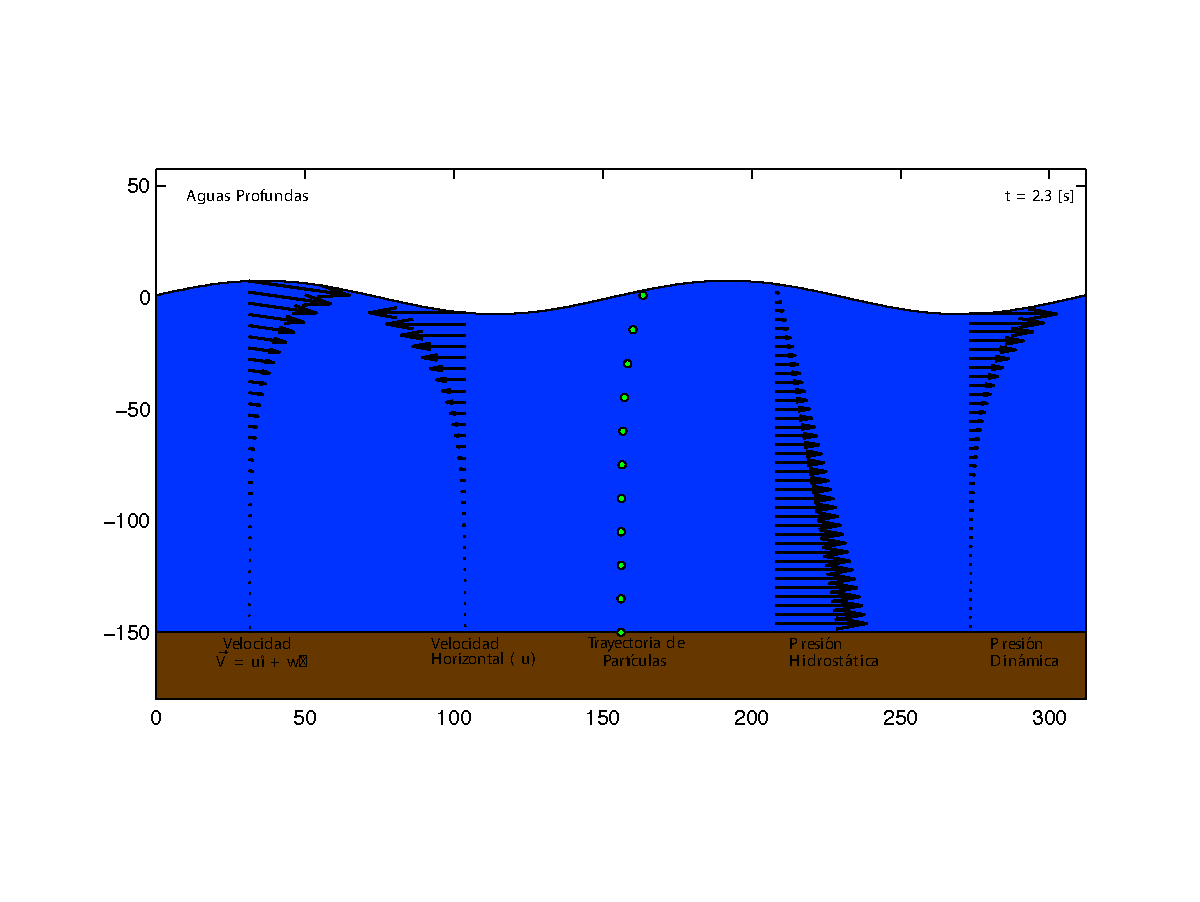
\includegraphics[scale=0.75]{figs/fig_1.pdf}
%\vspace{-4.5mm}
\captionof{figure}{Aguas Profundas}}

\vspace{0.75cm}
\subsubsection{Hipótesis de trabajo:}

\lipsum[17]

\vspace{0.5cm}
\subsubsection{Objetivos generales y específicos:}

Objetivo general: \\

\lipsum[18]

\vspace{0.5cm}

Objetivos específicos:

\blindenumerate[4]

\subsubsection{Materiales y Métodos} \label{sec:sec3}

\lipsum[19-21]

{\centering
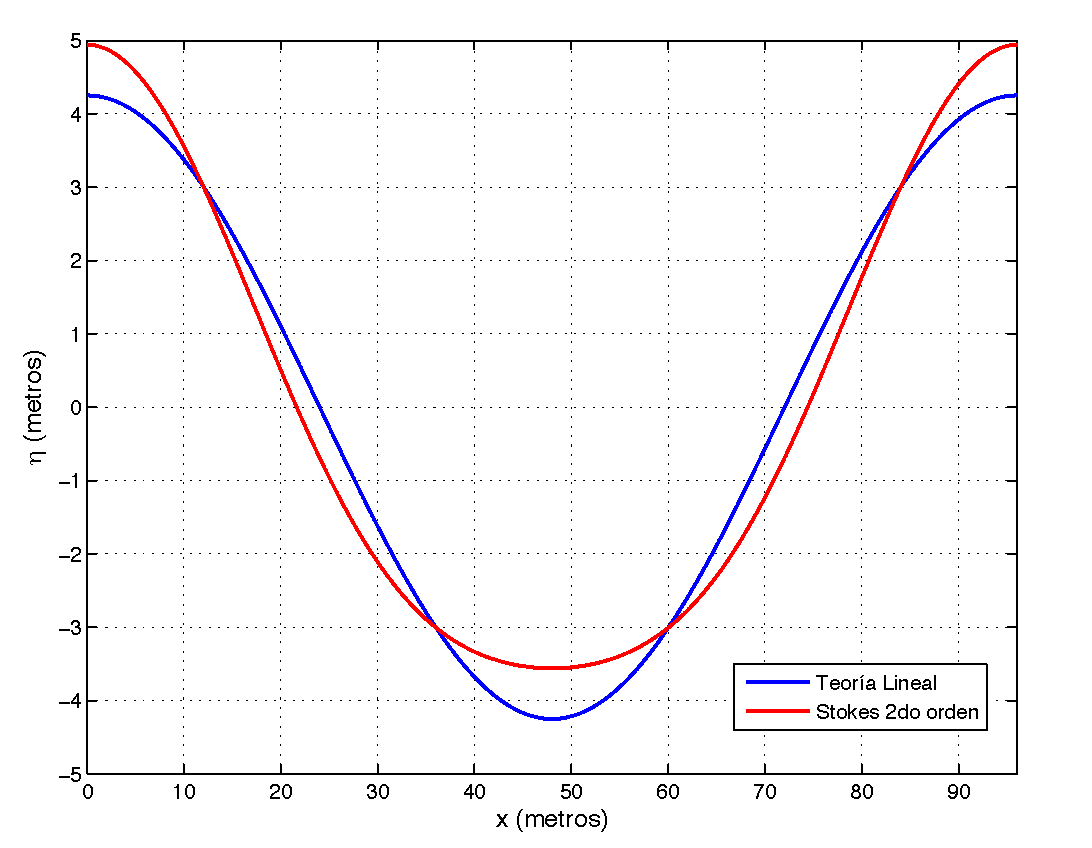
\includegraphics[scale=0.5]{figs/fig_6.pdf}
\vspace{-4.5mm}
\captionof{table}{Teoría lineal versus Stokes de segundo orden.}}
\vspace{3.5mm} 

\lipsum[22-25]


\subsubsection*{Stokes Drift}

\lipsum[26]

{\centering
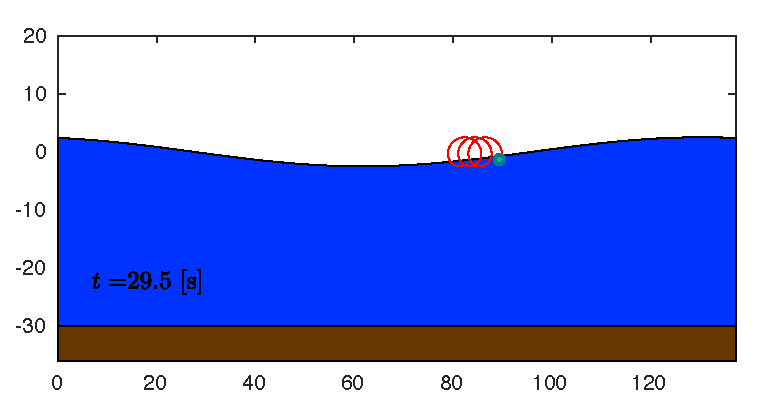
\includegraphics[scale=0.9]{figs/fig_2.pdf}
\vspace{-3.5mm}
\captionof{figure}{Simulación del Stokes Drift}}
\vspace{3.5mm}


%El análisis de las fuentes tsunamigénicas para distintos  eventos, generalmente se realiza mediante modelación numérica, a partir de series de tiempo de mareógrafos para las localidades en
%estudio. Para la simulación numérica se utilizan diversas mallas anidadas de diferente resolución espacial, a partir de diferentes fuentes de información, tales como GEBCO (General Bathymetric Chart of the Oceans), cartas náuticas y topografías de detalle. \\

\subsubsection*{Análisis de señales}

\lipsum[27]

\subsubsection*{Modelos numéricos de ondas largas}

\lipsum[28]


\subsubsection{Resultados Preliminares} \label{sec:sec4}

\lipsum[29-31]

{\centering
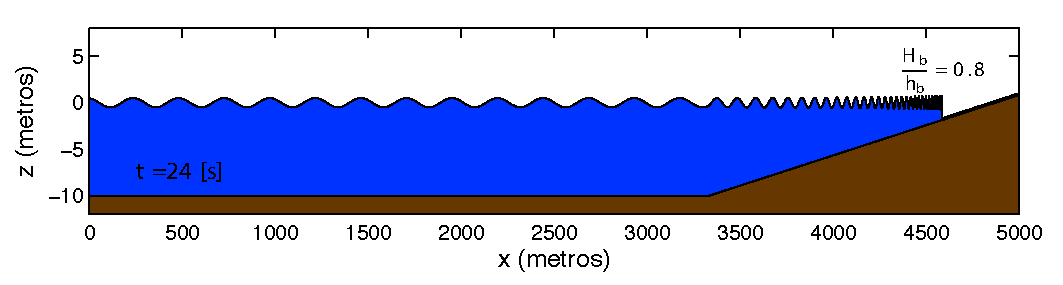
\includegraphics[scale=0.95]{figs/fig_3.pdf}
\vspace{-3.5mm}
\captionof{figure}{Teoría lineal sobre fondo plano y con pendiente.}}
\vspace{3.5mm}

\lipsum[22-35]

{\centering
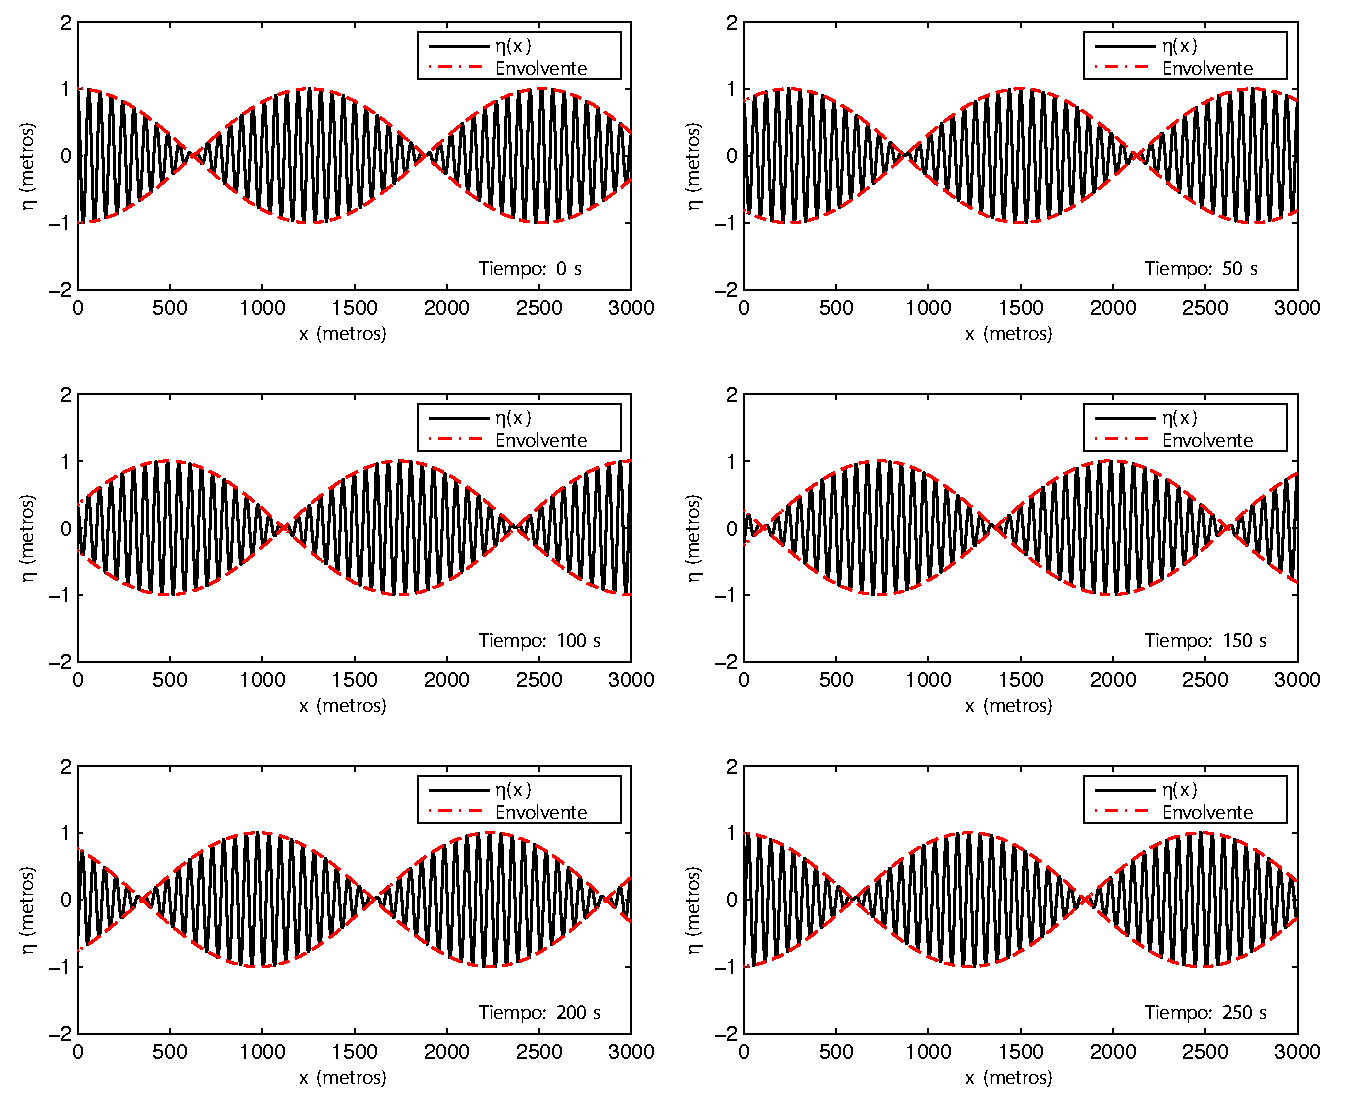
\includegraphics[scale=0.75]{figs/fig_4.pdf}
\vspace{-5mm}
\captionof{figure}{Snapshots Celeridad de Grupo.}}
\vspace{3.5mm}

\lipsum[36]

\subsubsection{Conclusión y Trabajo Futuro} \label{sec:sec5}

\lipsum[37-39]

\subsubsection*{Propuesta de publicaciones:}

\blindenumerate[3]

\subsubsection*{Agradecimientos} 

\lipsum[40]


\nocite{*}
%\addcontentsline
\renewcommand{\bibname}{Referencias}
\bibliographystyle{apa}
%\bibliographystyle{plain}
\bibliography{bibliografia}
%\addcontentsline{toc}{section}{Referencias}
\end{tcolorbox}


\newpage 

\subsection{INFRAESTRUCTURA DISPONIBLE.} Señale medios y recursos con que cuenta para realizar el proyecto. \textbf{La extensión máxima de esta sección es de media página con espaciamiento y tamaño de letra similares a los aquí usados. }

\begin{tcolorbox}[breakable]

\lipsum[41-42]

\end{tcolorbox}

\begin{tcolorbox}[breakable]
\textbf{Detalle ítems y montos globales que aporta el tutor:
} \\

\lipsum[43]

\blindenumerate[2]

\end{tcolorbox}

\newpage

\subsection{} Señale otros aspectos que Ud. considere relevantes para la evaluación del proyecto de tesis doctoral. \textbf{La extensión máxima de esta sección es de media página escrita con espaciamiento y tamaño de letra similar a los aquí usados.}

\begin{tcolorbox}[breakable]
Algunos aspectos importantes que se pueden mencionar acerca de la elaboración de este proyecto de tesis doctoral son:

\blindenumerate[5]

\end{tcolorbox}


\newpage

\section{PRESUPUESTO}

\subsection{RECURSOS DISPONIBLES:} Indique cuáles son los recursos que están concurriendo a financiar su tesis.

\begin{tcolorbox}[breakable]

\lipsum[44]

\blindenumerate[3]

\lipsum[45]

\end{tcolorbox}


\newpage 

\section{ANTECEDENTES CURRICULARES}
\subsection{DEL ESTUDIANTE}

\begin{enumerate}
\item  \textbf{ANTECEDENTES ACADEMICOS Y PROFESIONALES} \\
\begin{table}[h]
\taburowcolors[2]{white .. black!20}
\sffamily\footnotesize
\tabulinesep=6pt
\arrayrulewidth=1pt
\begin{tabu}{| X[lm] | X[lm]| X[0.5cm,lm] | X[0.5cm,lm] |}
\hline
\rowcolor{black!60}\color{white}\textbf{TITULOS/ GRADOS/CURSO (*)} & \color{white}\textbf{UNIVERSIDAD} &      \color{white}\textbf{PAÍS} & \color{white}\textbf{AÑO OBTENCIÓN} \\ \hline Licenciado en Ciencias de la Ingeniería & Universidad Católica de La Santísima Concepción & Chile & 2012 \\ \hline  Ingeniero Civil & Universidad Católica de La Santísima Concepción & Chile & 2015 \\ \hline
\end{tabu}
\end{table}

\item \textbf{TRAYECTORIA EN EL PROGRAMA DE DOCTORADO} \\
\textbf{(Debe adjuntar certificado de notas de los cursos realizados en el Programa de Doctorado, indicando semestre y año en que fue cursado y números de créditos).}
\item \textbf{PARTICIPACION DEL ESTUDIANTE EN OTROS PROYECTOS (En ejecución o finalizados) }\\ 
\begin{table}[h]
\taburowcolors[2]{white .. black!20}
\sffamily\footnotesize
\tabulinesep=6pt
\arrayrulewidth=1pt
\begin{tabu}{| X[0.2cm,lm] | X[0.2cm,lm] | X[lm]| X[0.5cm,lm] | X[0.5cm,lm] |}
\hline
%\rowcolor{black!60}
 
\multicolumn{2}{|c|}{\cellcolor{black!60}\color{white} \textbf{AÑO}} & \cellcolor{black!60}\color{white}\textbf{TÍTULO} & \cellcolor{black!60}\color{white}\textbf{FINANCIAMIENTO (origen y monto)} & \cellcolor{black!60}\color{white}\textbf{FUNCIONES DESEMPEÑADAS} \\ \hline  
Inicio & Término & &  & \\ \hline  
XXXX & XXXX & Centro de Investigación de Excelencia Nacional: Centro de Investigación para la Gestión Integrada del Riesgo de Desastres (CIGIDEN), Conicyt-FONDAP
N$^{\circ}$ 15110017.  & Beca Estudiante de Doctorado & Estudiante de Doctorado con participación activa en diversas áreas académicas y extra-académicas para el desarrollo y avance del conocimiento en temas de amenazas de tsunamis, y en general como personal de apoyo al centro.\\ \hline 
 & &  &  &  \\ \hline
\end{tabu}
\end{table}



\item \textbf{PUBLICACIONES IN EXTENSO.} Proporcione las referencias completa de los trabajos publicados, si los tiene. Por favor no incluya \textbf{resúmenes simples o expandidos}.
\begin{table}[h]
\taburowcolors[2]{white .. black!20}
\sffamily\footnotesize
\tabulinesep=6pt
\arrayrulewidth=1pt
\begin{tabu}{| X[lm] | X[lm] |}
\hline
\rowcolor{black!60}\color{white}\textbf{AUTORES Y TÍTULO} & \color{white}\textbf{REVISTA, VOLUMEN, PÁGINA INICIAL, FINAL, AÑO} \\ \hline
 &  \\ \hline
    & \\ \hline
\end{tabu}
\end{table}

\newpage

\item \textbf{PRESENTACIONES A CONGRESO:} Si lo desea, incluya información sobre \textbf{5 presentaciones a Congresos}. \\
\begin{table}[h]
\taburowcolors[2]{white .. black!20}
\sffamily\footnotesize
\tabulinesep=6pt
\arrayrulewidth=1pt
\begin{tabu}{| X[lm] | X[lm]| X[lm] |}
\hline
\rowcolor{black!60}\color{white}\textbf{TITULO} & \color{white}\textbf{CONGRESO} &      \color{white}\textbf{LUGAR/FECHA} \\ \hline
Quiroz M., Aránguiz R., Belmonte A. (2014). Peligro de tsunami en Chile central: Modelo de
ruptura del evento de 1730. & XXVI Congreso Latinoamericano de Hidráulica.  & Santiago, Chile. / Agosto 2014. \\ \hline  
Quiroz M., Aránguiz R. (2015). Modelación del tsunami de 1985 en Chile central. & XXII
Congreso Chileno de Ingeniería Hidráulica. & Santiago, Chile. / Octubre 2015.   \\ \hline        
Quiroz M., Álvarez G., León J., Cienfuegos R., Mas E. (2016). Analysis of micro-vulnerabilities in tsunami escape routes, case study, Iquique, Chile. & 3rd Young Coastal Scientists and
Engineers Conference – Americas. & Kingston, Canadá. / Junio 2016. \\ \hline
Aránguiz R., Quiroz M. (2016). Simulación numérica del tsunami de 1730 en el puerto de San Antonio. & VII Seminario Internacional de Ingeniería y Operación Portuaria  &  San Antonio, Chile. / Octubre 2016. \\ \hline
  &   &  \\ \hline
\end{tabu}
\end{table}
\end{enumerate}
\newpage

\vspace*{10mm}

\begin{center}
\textbf{CRITERIOS DE EVALUACIÓN}
\end{center} 
\vspace{5mm}

\textbf{I. INVESTIGACIÓN PROPUESTA}

\begin{enumerate}
\item Originalidad de la investigación y de las hipótesis de trabajo.
\item Claridad de la formulación del proyecto y de los objetivos planteados. 
\item Rigurosidad de la fundamentación teórica.
\item Claridad y pertinencia de la discusión bibliográfica.
\item Pertinencia de los métodos propuestos para obtener y validar resultados de acuerdo a los objetivos específicos.
\end{enumerate}

\textbf{II. VIABILIDAD DE EJECUCIÓN}

\begin{enumerate}
\item Coherencia entre el plan de trabajo, los objetivos específicos y los plazos propuestos. 
\item Pertinencia de los métodos propuestos para obtener y validar resultados de acuerdo a los objetivos específicos.
\item Adecuación de la infraestructura y financiamiento disponible a las necesidades del proyecto de tesis.
\end{enumerate}

\textbf{III. RELEVANCIA}

\begin{enumerate}
\item Relevancia de la investigación y contribución al conocimiento de la disciplina.
\end{enumerate}

\newpage

\begin{landscape}
\label{anexo}
\vspace*{5mm}
\hspace*{-15mm}
%\hspace*{-52.5mm}
\noindent\resizebox{1.325\textwidth}{!}{
    %\begin{figure}
    \begin{tikzpicture}[x=0.5cm, y=0.5cm]
     \begin{ganttchart}[%Specs
     y unit title=0.5cm,
     y unit chart=0.5cm,
     vgrid,hgrid,
     title height=1,
     progress=today,
     today=22,
%     title/.style={fill=none},
     title label font=\bfseries\footnotesize,
     bar/.style={fill=blue},
     bar height=0.7,
   %progress label text={picoo},
     group right shift=0,
     group top shift=0.7,
     group height=.3,
     group peaks width={0.2},
     inline]{1}{48}
    %labels
    \gantttitle{Programa de Doctorado en Ciencias de la Ingeniería}{48}\\  % title 1
    %\gantttitle[]{Año 20XX}{6}                 % title 2
    \gantttitle[]{Año 20XX}{12}
    \gantttitle[]{Año 20XX}{12}
    \gantttitle[]{Año 20XX}{12}
    \gantttitle[]{Año 20XX}{12} \\              
    \gantttitle{T1}{3}
    \gantttitle{T2}{3}
    \gantttitle{T3}{3}
    \gantttitle{T4}{3}
    \gantttitle{T1}{3}
    \gantttitle{T2}{3}
    \gantttitle{T3}{3}
    \gantttitle{T4}{3}
    \gantttitle{T1}{3}
    \gantttitle{T2}{3}
    \gantttitle{T3}{3}
    \gantttitle{T4}{3}
    \gantttitle{T1}{3} 
    \gantttitle{T2}{3}
    \gantttitle{T3}{3} 
    \gantttitle{T4}{3}\\
    % Setting group if any
    \ganttgroup[inline=false]{Cursos Optativos}{1}{18}\\ 
    \ganttbar[progress=100,inline=false]{Planificación}{1}{18}\\

    \ganttgroup[inline=false]{Cursos CPD}{13}{30} \\ 
    \ganttbar[progress=87,inline=false]{Planificación}{7}{21} \\
    
    \ganttgroup[inline=false]{Proyecto de Tesis}{1}{24} \\ 
    \ganttbar[progress=100,inline=false]{I}{1}{6} \\
    \ganttbar[progress=100,inline=false]{II}{7}{12} \\
    \ganttbar[progress=75,inline=false]{III}{13}{18} \\
    \ganttbar[progress=45,inline=false]{IV}{19}{24} \\
    %\ganttmilestone[inline=false]{Milestone 3}{22} \\      

    \ganttgroup[inline=false]{Tesis de Doctorado}{25}{42} \\ 
    \ganttbar[progress=0,inline=false]{I}{25}{30} \\
    \ganttbar[progress=0,inline=false]{II}{31}{36}\\ 
    \ganttbar[progress=0,inline=false]{III}{37}{42}\\     
    %\ganttbar[progress=50,inline=false, bar progress label node/.append style={below left= 10pt and 7pt}]{II}{13}{24} \\ \\
    %\ganttmilestone[inline=true]{AAS}{22} \\ 
 
    %\ganttbar[progress=70,inline=false]{Task D}{18}{20} \\
    
    \ganttgroup[inline=false]{Pasantía}{37}{42} \\ 
    \ganttbar[progress=0,inline=false]{Planificación}{31}{36} \\ 

    \ganttgroup[inline=false]{Revisión Bibliográfica}{1}{24} \\ 
    \ganttbar[progress=85,inline=false]{Tema 1}{1}{12} \\     
    \ganttbar[progress=60,inline=false]{Tema 2}{13}{24} \\     
    
    \ganttgroup[inline=false]{Análisis de Datos}{13}{24} \\ 
    \ganttbar[progress=100,inline=false]{Procesamiento}{13}{18} \\  
    \ganttbar[progress=60,inline=false]{Simulaciones Numéricas}{10}{26} \\
    \ganttbar[progress=30,inline=false]{Análisis Discreto}{16}{30} \\
    \ganttbar[progress=15,inline=false]{Análisis Espectral}{18}{32} \\
    \ganttbar[progress=20,inline=false]{Wavelets Analysis}{18}{34} \\          

    \ganttgroup[inline=false]{Resultados y Conclusiones}{22}{46} \\ 
    \ganttbar[progress=0,inline=false]{Análisis Crítico}{22}{42} \\  
    \ganttbar[progress=0,inline=false]{Validez}{46}{48}   \\ 
    \ganttbar[progress=0,inline=false]{Aporte al Conocimiento}{42}{46}   \\ 

\ganttgroup[inline=false]{Papers}{25}{39} \\ 
    \ganttbar[progress=0,inline=false]{Artículo 1}{25}{30} \\  
    \ganttbar[progress=0,inline=false]{Artículo 2}{34}{39}    \\
    
    \ganttgroup[inline=false]{Redacción Memoria}{37}{48} \\ 
    \ganttbar[progress=0,inline=false]{Escritura}{37}{46} \\  
    \ganttbar[progress=0,inline=false]{Defensa Tesis}{46}{48}   
\end{ganttchart}
    %\caption{Diagrama Gantt Para}
\node[above,font=\large\bfseries] at (current bounding box.north) {ANEXO: PLAN DE TRABAJO};    
\end{tikzpicture}
%\end{figure}
}
    \captionof{figure}{Diagrama Gantt estimando el avance de investigación tentativo, generado por el alumno. Las barras delgadas (naranjas) representan el avance teórico del alumno sujeto al plan de estudios sugerido por la dirección de postgrado. Las barras más gruesas (azules) representan el avance efectivo realizado por el alumno Marco Quiroz.}

\end{landscape}

%\newpage

%\begin{sidewaysfigure}[ht]
%\centering
%\includegraphics[scale=0.85]{gantt.pdf}
%\end{sidewaysfigure}

\end{document}